\section{}

\textbf{Tiempo de lectura:} \{s03-reading-time\}

La historia de los sistemas operativos se puede dividir en cinco grandes
etapas o generaciones, obviamente conectadas con las generaciones de los
ordenadores donde funcionaban.

\section{1ª Generación
(1945-55)}\label{sect-historia-primera-generaciuxf3n}

En la primera generación de ordenadores no se utilizaban sistemas
operativos.

Sus principales características son:

\begin{itemize}
\item
  Computadoras construidas con electrónica de
  \href{https://es.wikipedia.org/wiki/V\%C3\%A1lvula_termoi\%C3\%B3nica}{válvulas
  de vacío}.
\item
  Sin sistema operativo.
\item
  Sin lenguajes de programación. Se programaban directamente en lenguaje
  máquina.
\end{itemize}

Algunos ejemplos de ordenadores destacables fueron:

\begin{description}
\item[\href{https://es.wikipedia.org/wiki/ENIAC}{ENIAC} (1945)]
Se le considera el primer ordenador electrónico digital de propósito
general, aunque existe cierta polémica sobre este punto. Lo cierto es
que se construyeron otros ordenadores antes que este, pero o no eran de
propósito general ---como las famosas computadoras
\href{https://es.wikipedia.org/wiki/Colossus}{Colossus} (1944), que
fueron diseñadas para ayudar en
\href{https://es.wikipedia.org/wiki/Criptoan\%C3\%A1lisis}{criptoanálisis}---
o no eran electrónicos sino electromecánicos ---como la computadora
\href{https://es.wikipedia.org/wiki/Z3}{Z3} (1941), que usaba
\href{https://es.wikipedia.org/wiki/Rel\%C3\%A9}{relés}---.

No era un producto comercial sino un proyecto experimental de defensa
que principalmente se diseñó y utilizó para calcular tablas de tiro de
artillería destinadas al Laboratorio de Investigación Balística del
Ejército de los Estados Unidos.

\href{https://es.wikipedia.org/wiki/Z4}{Z4} (1945) fue el primer
ordenador digital comercial, pero era electro-mecánico.
\item[\href{https://es.wikipedia.org/wiki/IBM_701}{IBM 701} (1953)]
Fue el primer \emph{mainframe} de la serie IBM 700, que a la larga se
convertiría en un éxito de ventas. Utilizaba tubos de vacío y tarjetas
perforadas.
\end{description}

El IBM 7090 ---versión transistorizada del 709, que utilizaba válvulas
de vacío, como todos los de la serie 700--- y el posterior 7094, fueron
usados por la NASA para los cálculos de control de las misiones de los
programas espaciales Mercury y Gemini y durante la primera etapa del
programa Apolo.

\section{2ª Generación
(1955-64)}\label{sect-historia-segunda-generaciuxf3n}

En la segunda generación de ordenadores los transistores reemplazaron a
las válvulas de vacío.

En lo que respecta a los sistemas operativos:

\begin{itemize}
\item
  Aparecen los monitores del sistema, que se pueden considerar un
  predecesor de los sistemas operativos.
\item
  Sistema de procesamiento por lotes.
\item
  Se comienzan a utilizar lenguajes de programación, como: ensamblador,
  FORTRAN y COBOL.
\end{itemize}

\href{https://es.wikipedia.org/wiki/GM-NAA_I/O}{GM-NAA I/O}
(\emph{General Motors and North American Aviation Input/Output system})
fue el primer sistema operativo. Fue desarrollado por General Motors
Research Laboratory en 1956 para el \emph{mainframe}
\href{https://en.wikipedia.org/wiki/IBM_704}{IBM 704} con el fin de
automatizar la carga y ejecución de un nuevo trabajo una vez había
terminado el anterior. Para su desarrollo se basaron en un monitor del
sistema creado en 1955 por programadores de General Motors para el IBM
701.

\begin{figure}
\centering
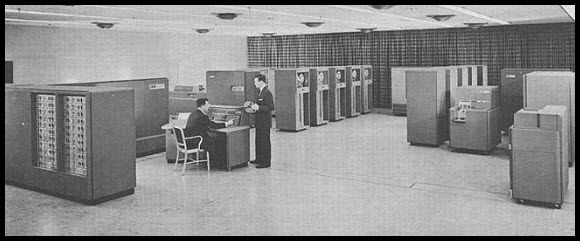
\includegraphics[keepaspectratio]{media/C03_historia/instalación_ibm_702.jpg}
\caption{Instalación de un mainframe IBM 702 --- Fuente:
\href{https://commons.wikimedia.org/wiki/File:BRL61-IBM_702.jpg}{Wikipedia}}\label{fig-instalaciuxf3n-ibm-702}
\end{figure}

\section{3ª Generación
(1965-1968)}\label{sect-historia-tercera-generaciuxf3n}

En la tercera generación se comenzaron a utilizar los circuitos
integrados, que fue una invención de finales de la década de 1950.

En lo que respecta a los sistemas operativos:

\begin{itemize}
\item
  Aparecen los sistemas operativos multiprogramados.
\item
  Aparecen más lenguajes de programación.
\end{itemize}

El ejemplo más destacado de esta época es el \{ibmos360\} Fue un sistema
operativo desarrollado por IBM para su \emph{mainframe}
\href{https://en.wikipedia.org/wiki/IBM_System/360}{IBM System/360}
(S/360) (véase la
\hyperref[fig-instalaciuxf3n-ibm-system-360]{Instalación de un mainframe
IBM System/360 --- Fuente: }). Su versión DOS/360 (\emph{Disk Operating
System/360}) fue el primer sistema operativo en hacer los discos
magnéticos un requisito para poder operar.

\begin{figure}
\centering
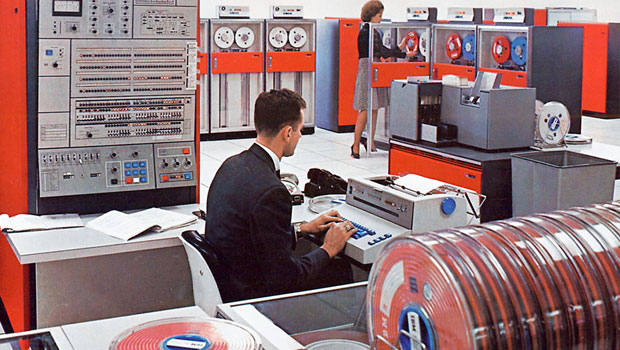
\includegraphics[keepaspectratio]{media/C03_historia/instalación_ibm_system_360.jpg}
\caption{Instalación de un mainframe IBM System/360 --- Fuente:
\href{https://www.ibm.com/history/system-360}{IBM}}\label{fig-instalaciuxf3n-ibm-system-360}
\end{figure}

Se anunció en 1964, pero fue lanzado en 1966, con un año de retraso
respecto a la fecha prevista originalmente. Los motivos fundamentales
fueron ciertos problemas de organización interna de la compañía y la
falta de experiencia en proyectos de esa envergadura. Las previsiones
iniciales eran de 1 millón de líneas de código y miles de componentes de
software.

Algunos autores fechan los inicios de la ingeniería del software en la
publicación del libro «The Mythical Man-Month: Essays on Software
Engineering», escrito por Frederick Brooks y publicado en 1975.
Frederick Brooks se basó en la experiencia adquirida mientras
administraba el desarrollo del IBM OS/360, donde era jefe de proyecto.

\section{4ª Generación
(1965-1980)}\label{sect-historia-cuarta-generaciuxf3n}

La cuarta generación abarca desde mediados de los años 60 hasta finales
de la década de los 70. Respecto a los ordenadores, es el resultado del
desarrollo de los microprocesadores.

En lo que respecta a los sistemas operativos:

\begin{itemize}
\item
  Aparecen los sistemas operativos de tiempo compartido.
\item
  Aparecen los terminales, los programas interactivos y las máquinas
  virtuales.
\end{itemize}

A continuación veremos los ejemplos más representativos de esta época.

\subsection{MULTICS}\label{_multics}

\href{https://es.wikipedia.org/wiki/Multics}{MULTICS} fue anunciado en
1964, fruto de la colaboración entre el MIT, General Electrics y Bell
Labs, como el primer sistema operativo de propósito general.

\begin{figure}
\centering
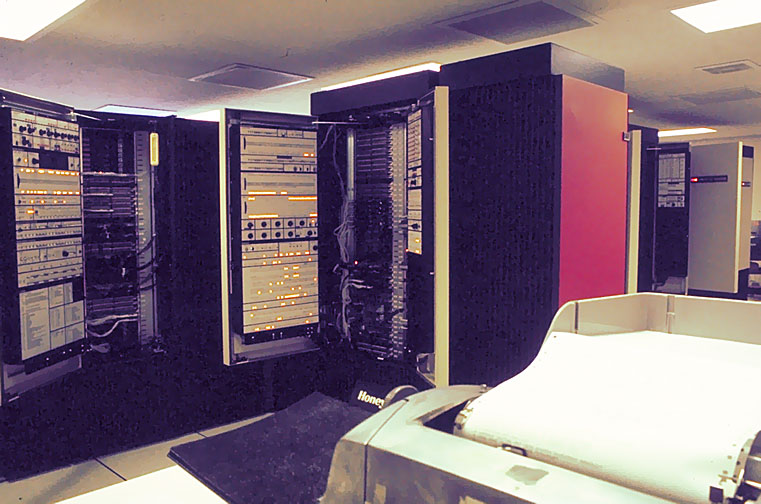
\includegraphics[keepaspectratio]{media/C03_historia/multics_mainframe.jpg}
\caption{Mainframe GE-6180 con sistema MULTICS, en torno a 1976 en el
MIT --- Fuente:
\href{http://www.multicians.org/multics-stories.html}{Multicians}}\label{sect-multics-mainframe}
\end{figure}

Fue el primer sistema operativo en proporcionar un sistema de archivos
jerárquico, intérprete de comandos implementado como programa de
usuario, listas de control de acceso individuales para cada archivo y
enlazado dinámico, entre otras características novedosas.

Además experimentó con eliminar la separación entre el espacio de
direcciones de los procesos y los archivos. Es decir, como si los
archivos estuvieran mapeados en memoria, permitiendo a los procesos
acceder al contenido de los archivos directamente, sin tener que ordenar
manualmente operaciones de lectura desde el disco a la memoria (véase el
\hyperref[_archivos_mapeados_en_memoria]{???}).

\subsection{VM/CMS}\label{_vmcms}

\href{https://es.wikipedia.org/wiki/VM_(sistema_operativo)}{VM/CMS} es
un sistema de IBM utilizado en los \emph{mainframes}
\href{https://en.wikipedia.org/wiki/IBM_System/360}{IBM System/360},
System/370, System/390 y zSeries. VM es un
\href{https://es.wikipedia.org/wiki/Hipervisor}{hipervisor} que se
encarga de virtualizar el hardware para crear múltiples máquinas
virtuales, dando la sensación de que cada una es un \emph{mainframe}
independiente.

Como sistema operativo de las máquinas virtuales, una opción común es
CMS, un sistema interactivo y monousuario muy ligero, diseñado para
operar fundamentalmente en una máquina virtual de VM. Gracias a VM/CMS,
cada usuario tiene la sensación de trabajar en un sistema completamente
independiente y seguro.

El desarrollo de VM/CMS comenzó en 1965 y la primera versión estuvo
disponible a primeros de 1966. Las versiones actuales se denominan IBM
z/VM.

\subsection{UNIX}\label{_unix}

\{unix\} fue desarrollado originalmente por Bell Labs en 1970 para los
sistemas \href{https://es.wikipedia.org/wiki/PDP-11}{PDP-11/20} (véase
la \hyperref[fig-dec-pdp11]{Dennis Ritchie (de pie) y Ken Thompson
(sentado) frente a un PDP-11 y sus dos terminales  --- Fuente: }). La
autoría de este se le atribuye a un grupo de programadores, liderados
por Ken Thompson, que decidieron rehacer el trabajo de MULTICS, pero a
menor escala, después de que Bell Labs abandonara el proyecto MULTICS en
1969. Inicialmente se llamó UNICS y fue desarrollado para los sistemas
PDP-7 ---una minicomputadora de la serie PDP de Digital Equipment
Corporation (DEC)---.

\begin{figure}
\centering
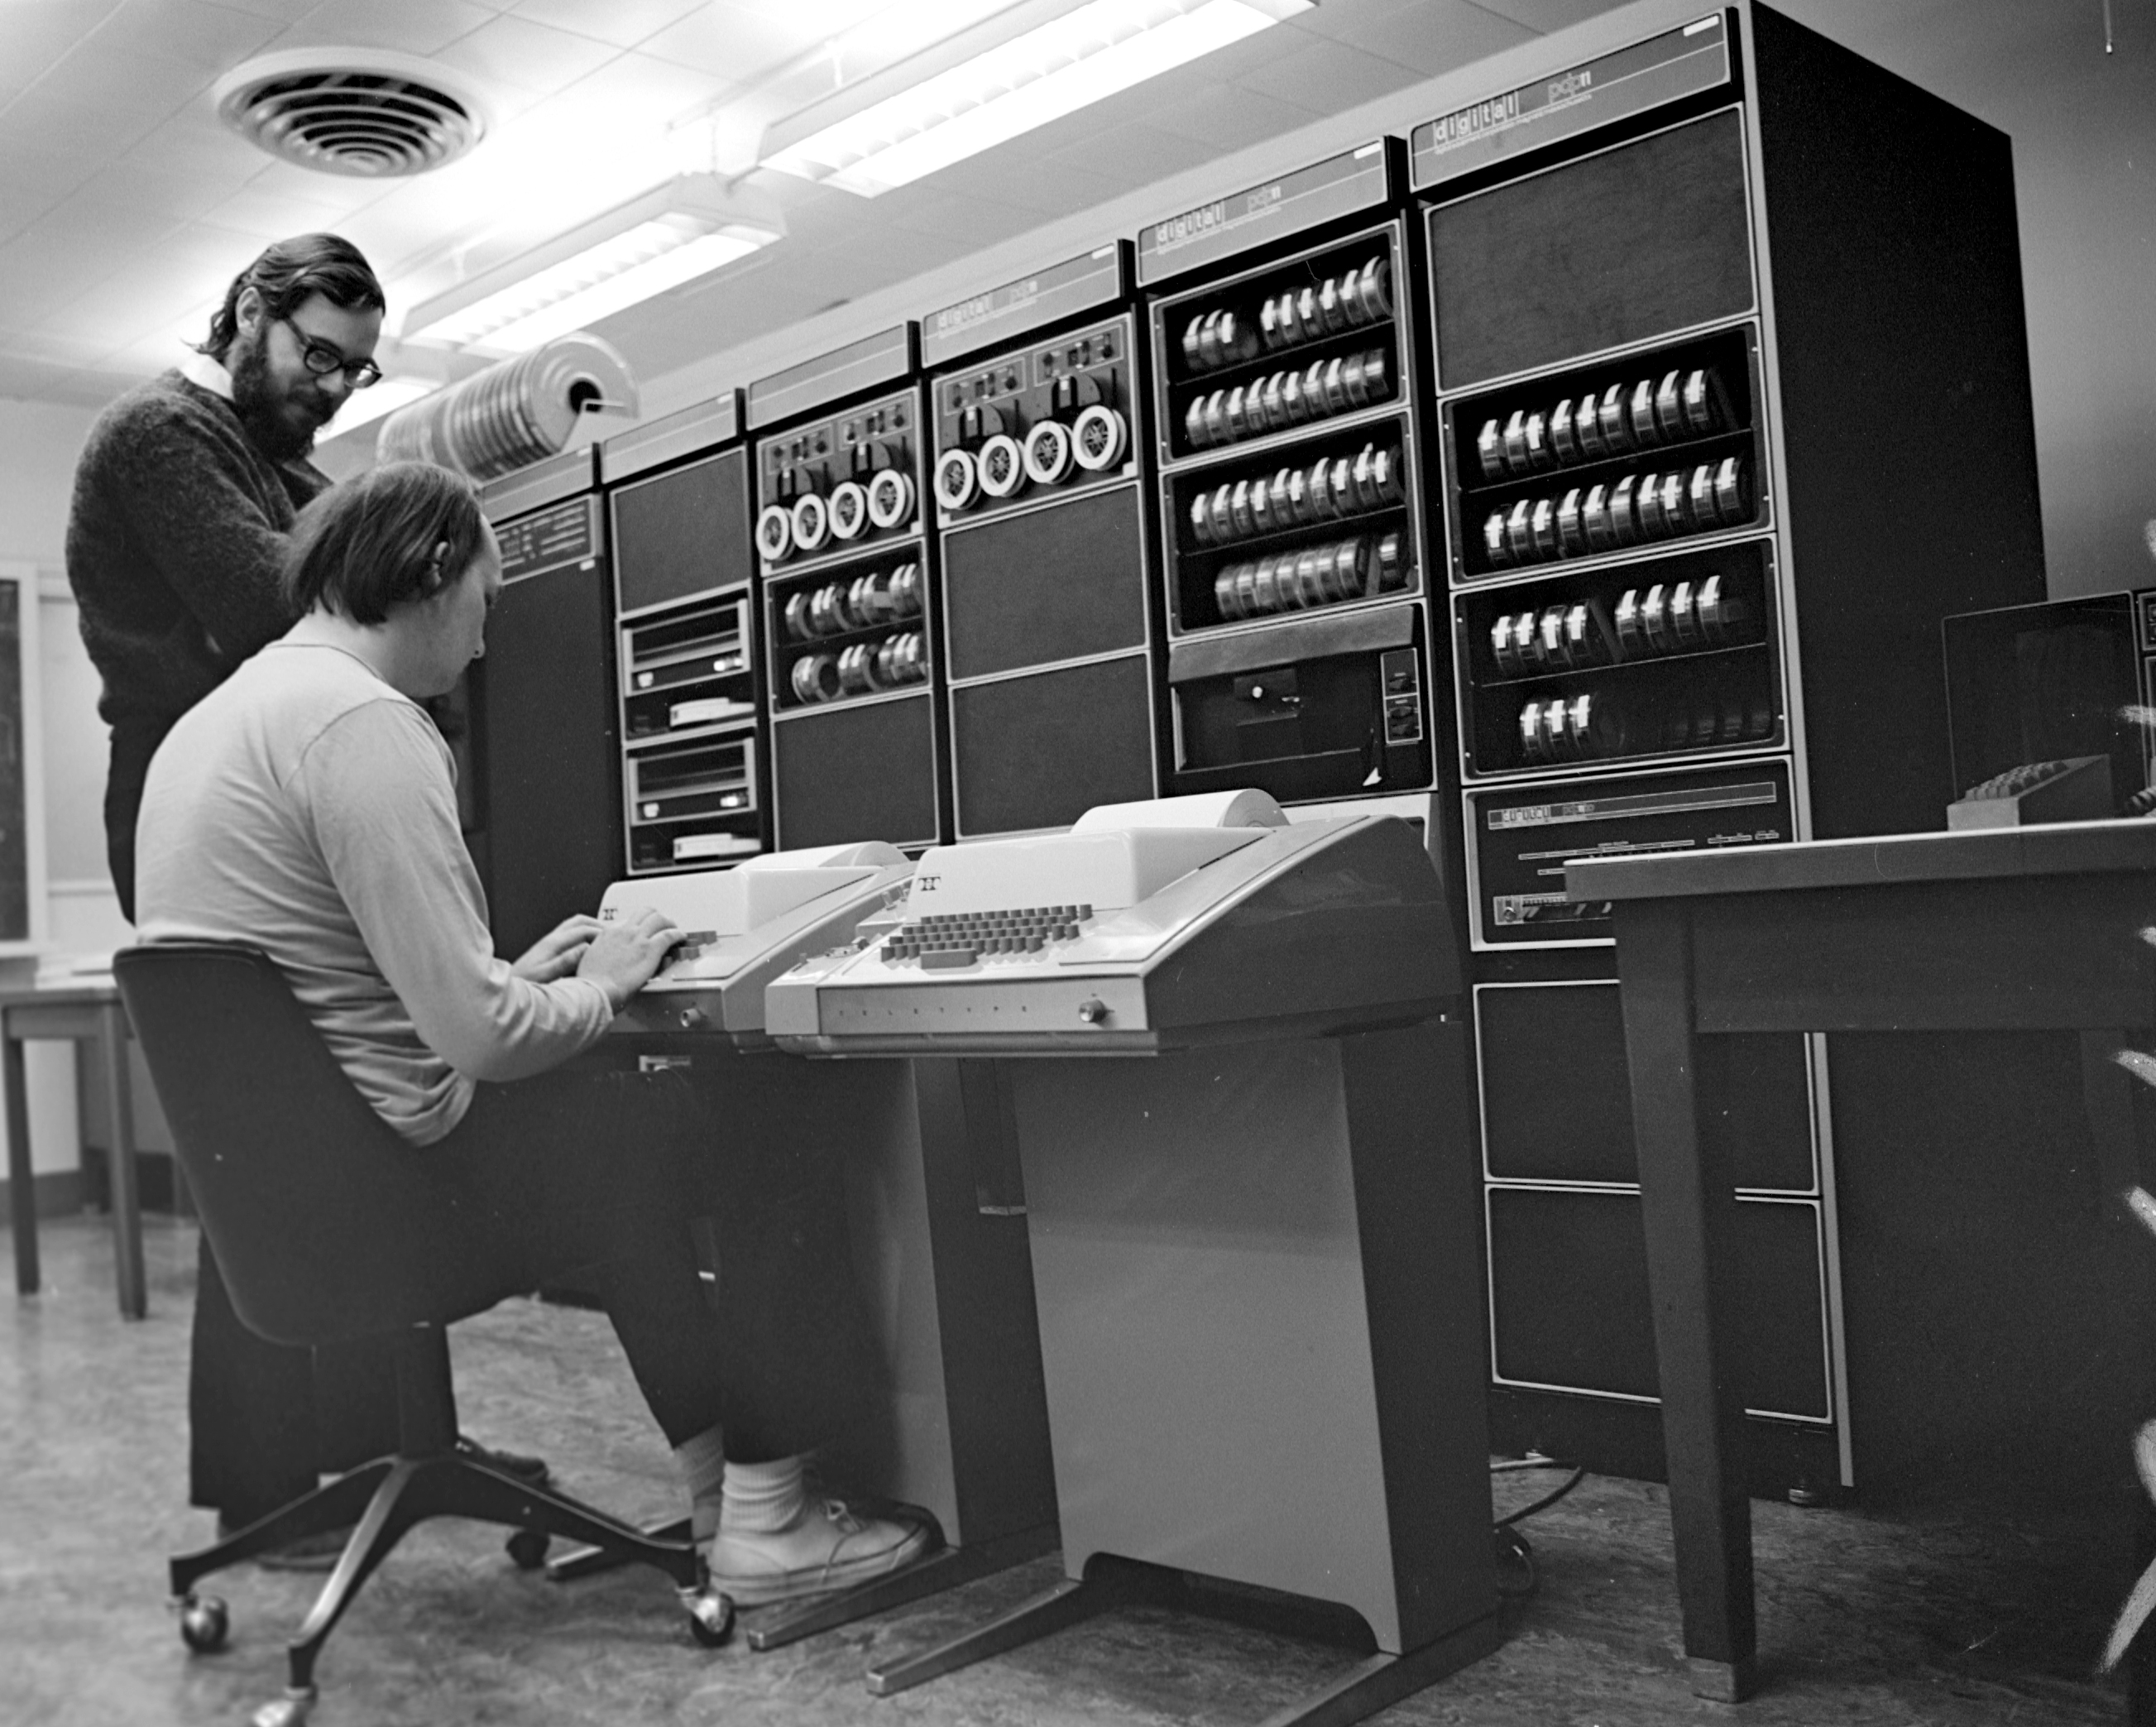
\includegraphics[keepaspectratio]{media/C03_historia/dec_pdp11_ken_den.jpg}
\caption{Dennis Ritchie (de pie) y Ken Thompson (sentado) frente a un
PDP-11 y sus dos terminales
\href{https://en.wikipedia.org/wiki/Teletype_Model_33}{Teletype
33} --- Fuente: \href{https://www.bell-labs.com/usr/dmr/www/}{Dennis
Ritchie}}\label{fig-dec-pdp11}
\end{figure}

Los sistemas UNIX se caracterizan por ofrecer un gran número de pequeñas
herramientas especializadas diseñadas para trabajar unidas ---a través
de la línea de comandos usando tuberías--- y por usar la E/S salida de
archivos como modelo universal de E/S. Es decir, que los dispositivos,
ciertos mecanismos de comunicación entre procesos y hasta algunos
aspectos de la configuración e información del sistema son gestionados
como archivos.

La primera versión de UNIX fue implementada en ensamblador, como era
común en la época. Posteriormente, Dennis Ritchie y Brian Kernighan
diseñaron un nuevo lenguaje de programación llamado «C», especialmente
pensado para que UNIX fuera escrito con él. Eso facilitó que UNIX
pudiera ser portado a ordenadores diferentes. Además, gracias al
lenguaje C, el código era más conciso y compacto, lo que se tradujo en
que se pudieron desarrollar nuevas funcionalidades más rápidamente.

AT\&T, la compañía matriz de Bell Labs, no podía competir en la
industria de los ordenadores, por lo que puso el código fuente de UNIX a
disposición de universidades, compañías privadas y del gobierno de los
Estados Unidos. Eso aumentó su difusión y dio resultados inesperados.
Por ejemplo, una de las variantes más importantes de UNIX fue \{bsd\},
desarrollada por la Universidad de California en Berkeley.

La versión 4.2BSD (\emph{Berkeley Software Distribution}) de esta
variante de UNIX fue la primera que incluyó la interfaz de
\emph{sockets} para facilitar la comunicación entre procesos a través de
Internet y otras redes. Esta interfaz se ha convertido en estándar en
prácticamente cualquier sistema operativo.

También implementó y ayudó a difundir el estándar de comunicaciones
TCP/IP, base de la actual Internet. Muchos sistemas operativos actuales,
tanto libres como privativos, utilizan código de UNIX BSD en sus
implementaciones de los protocolos TCP/IP y de diversas utilidades de
red.

\subsubsection{Familias}\label{_familias}

Los sistemas UNIX siguieron evolucionando hasta adaptarse a la 5ª
generación de sistemas, la de los sistemas de escritorio y los
ordenadores personales. En la actualidad se considera que hay dos
grandes familias de UNIX y las distintas variantes pertenecen a una u
otra en función del UNIX del que derivaron originalmente:

\begin{itemize}
\item
  La familia derivada de \textbf{AT\&T UNIX System V}, en la que se
  incluyen sistemas operativos no libres, tales como:
  \href{https://es.wikipedia.org/wiki/SCO_OpenServer}{SCO OpenServer},
  \href{https://es.wikipedia.org/wiki/Solaris_(sistema_operativo)}{Oracle/Sun
  Microsystems Solaris Operating Environment} y
  \href{https://es.wikipedia.org/wiki/UnixWare}{SCO UnixWare}.
\item
  La familia derivada de \textbf{UNIX BSD}, en la que se incluyen
  sistemas libres como: \{freebsd\},
  \href{https://es.wikipedia.org/wiki/NetBSD}{NetBSD},
  \href{https://es.wikipedia.org/wiki/OpenBSD}{OpenBSD}, \{darwin\} y
  \href{https://es.wikipedia.org/wiki/DragonFly_BSD}{DragonFly BSD},
  entre muchos otros.
\end{itemize}

\{freebsd\} es el sistema base de algunos sistemas no libres. Por
ejemplo, \{darwin\} es el sistema operativo en el que se basan los
sistemas operativos de Apple: macOS, IOS, watchOS, tvOS e iPadOS. A su
vez Darwin utiliza múltiples elementos de FreeBSD (véase el
\hyperref[_mach]{Mach}).

Otro ejemplo destacable es
\href{https://en.wikipedia.org/wiki/PlayStation_4_system_software}{Orbis
OS} ---el sistema operativo de PlayStation 4--- que también está basado
en FreeBSD.

\subsubsection{Estandarización}\label{_estandarizaciuxf3n}

En 1988 el \{ieee\} publicó el primer estándar \{posix\}, un intento de
crear un estandarizar mínimo de las características que debería soportar
cualquier sistema operativo. Este estándar se basó en las
características de las principales variantes de UNIX en el momento.

A principios de los 90, como las distintas variantes de UNIX estaban
divergiendo ---haciendo muy difícil desarrollar programas compatibles
con todas ellas--- se inició un esfuerzo para desarrollar una
especificación común; de tal forma que solo aquellas variantes que la
cumplieran pudieran denominarse como «UNIX». En 1994 se publicó la
\href{https://es.wikipedia.org/wiki/Single_Unix_Specification}{Single
UNIX Specification (SUR)}, gestionada por
\href{https://es.wikipedia.org/wiki/The_Open_Group}{The Open Group}.

En 1998, las organizaciones IEEE, The Open Group y la
\href{https://en.wikipedia.org/wiki/International_Organization_for_Standardization}{International
Organization for Standardization (ISO)} comenzaron a trabajar en una
nueva especificación que integrara POSIX y SUR. En 2002 se publicó como
la «Single UNIX Specification, Version 3», cuya base es idéntica al
estándar POSIX.1-2001 IEEE. Los sistemas operativos certificados por su
cumplimiento reciben la marca «UNIX 03», como es el caso de macOS. Pero
hay que tener en cuenta que la mayoría de los sistemas basados en UNIX
BSD y Linux no han pasado nunca por el proceso de certificación, por lo
que no pueden usar la marca UNIX, aunque cumplan con el estándar POSIX,
que es la base de la especificación SUR.

Desde 2002 se han publicado otras versiones de SUR, siempre sobre la
base de nuevas versiones de la especificación POSIX.

\subsubsection{Sucesores}\label{_sucesores}

Sistemas UNIX y estilo UNIX hay muchos, pero \{plan9\} ---también de
Bell Labs--- fue desarrollado para llevar los conceptos de UNIX un poco
más lejos, sustituyendo a UNIX en Bell Labs como plataforma principal de
investigación en sistemas operativos.

Plan 9 es un sistema operativo distribuido, diseñado para que una red
heterogénea de ordenadores separados geográficamente funcionara como un
único sistema informático. En Plan 9, cada proceso tiene su propia vista
del sistema de archivos, a través de la cual los procesos pueden acceder
a distintos recursos o comunicarse con otros procesos. Es decir, Plan 9
generalizó el modelo universal de E/S de UNIX ---basado en la E/S de
archivos--- porque todo a lo que puede tener acceso un proceso
---incluidos los canales de comunicación con otras aplicaciones y
servicios--- son archivos en la vista privada que del sistema de
archivos tiene cada proceso.

Los procesos en equipos diferentes pueden comunicarse de forma
transparente. Solo hace falta que un proceso exponga parte de su sistema
de archivos en la vista de los procesos que quieren comunicarse con él.
Esto ocurre de forma transparente, gracias al protocolo de comunicación
9P de Plan 9. Este protocolo es el que usan actualmente Windows
Subsystem for Linux (WSL), QEMU y otras herramientas de virtualización,
para ofrecer acceso a los archivos de una máquina virtual desde el
sistema operativo anfitrión.

El desarrollo de Plan 9 dejo otras aportaciones. Por ejemplo, el
estándar de codificación Unicode
\href{https://es.wikipedia.org/wiki/UTF-8}{UTF-8} nació para ser usado
en Plan 9 como formato de cadenas nativo.

En 1996, el desarrollo de Plan 9 pasó a un segundo plano para dar
prioridad a \{inferno\}, con el que Bell Labs intentó usar su
experiencia con Plan 9 para desarrollar un sistema operativo distribuido
que al mismo tiempo fuera una plataforma con la que competir con Java.
Las aplicaciones se desarrollaban en un lenguaje llamado Limbo y se
ejecutaban en una máquina virtual ---similar a la de Java--- que venía
incluida con Inferno. De esta manera las aplicaciones podían ejecutarse
independientemente de la arquitectura del hardware.

\subsection{VMS}\label{_vms}

\href{https://en.wikipedia.org/wiki/OpenVMS}{VMS} es un sistema
operativo de 32 bits diseñado originalmente por Digital Equipment
Corporation (DEC) ---ahora propiedad de HP--- en 1978 para usarlo en
minicomputadoras \href{https://es.wikipedia.org/wiki/VAX}{VAX}.
Posteriormente fue portado a sistemas DEC Alpha e Intel Itanium.

\begin{figure}
\centering
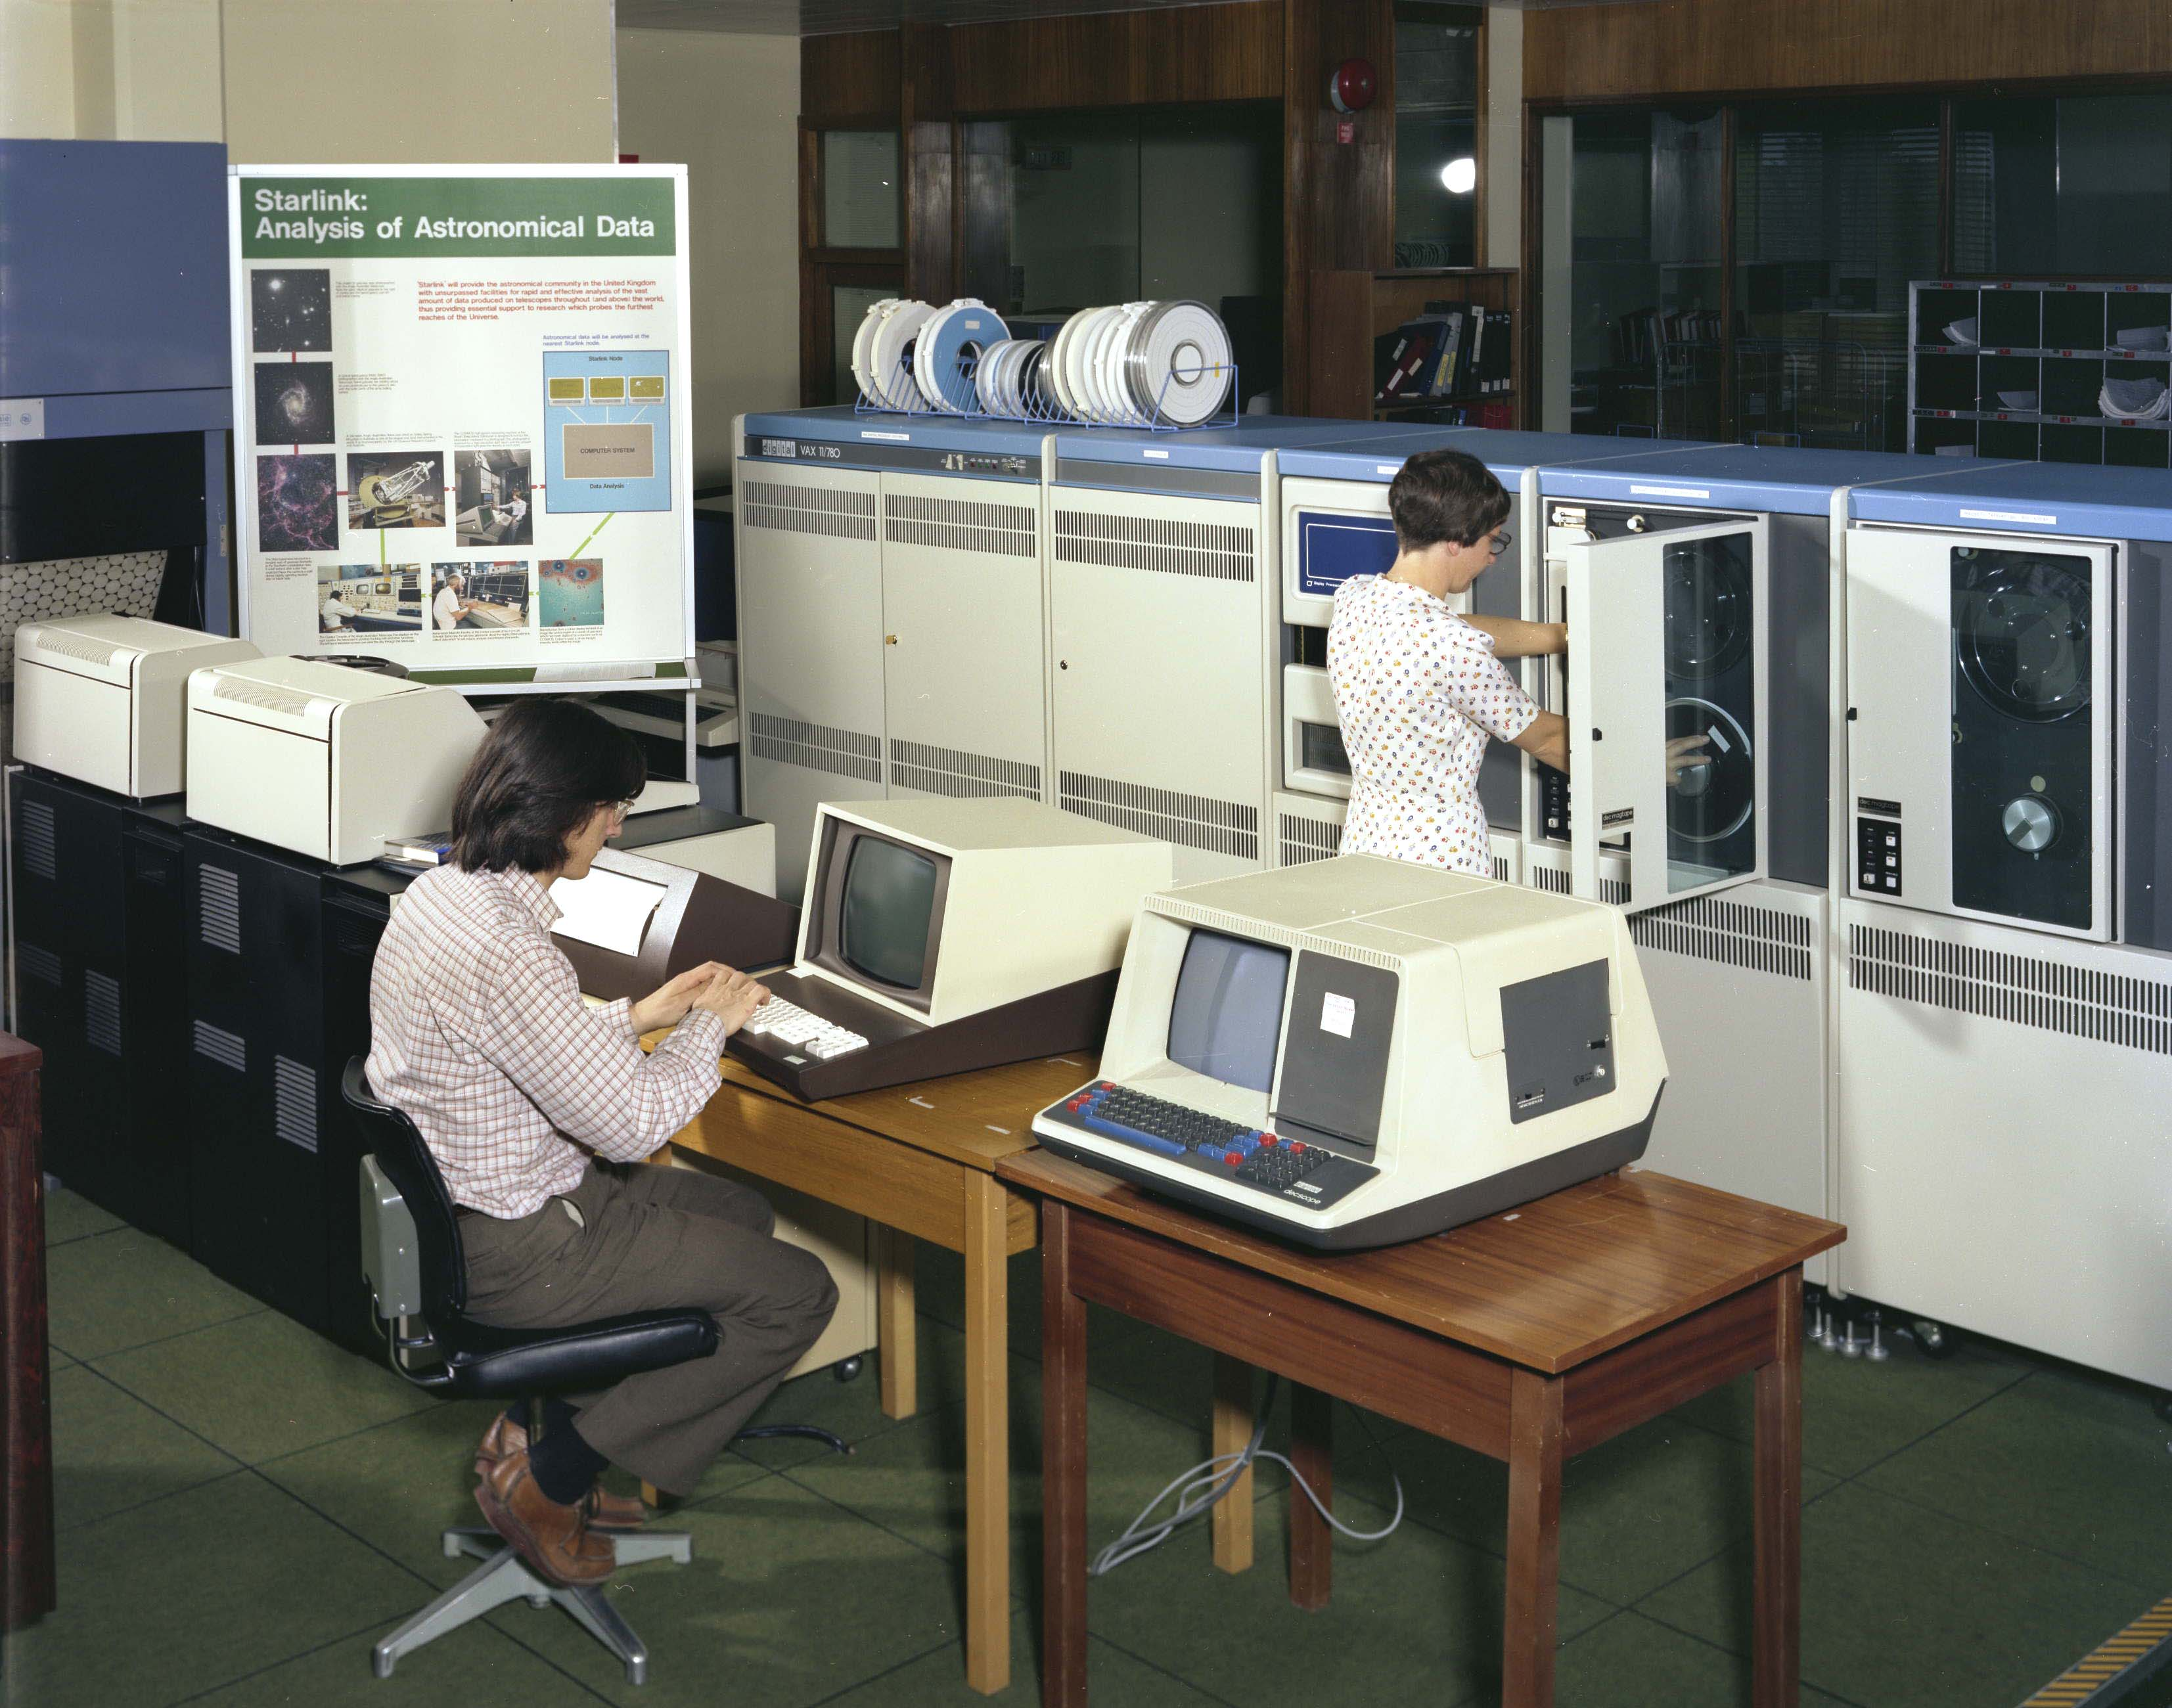
\includegraphics[keepaspectratio]{media/C03_historia/dec_vax11.jpg}
\caption{Instalación de VAX 11/780 en 1980 --- Fuente:
\href{http://www.chilton-computing.org.uk/}{Science and Technology
Facilities Council}}\label{fig-dec-vax11}
\end{figure}

Las siglas VMS vienen de \emph{Virtual Memory System}, ya que una de sus
principales características era explotar el concepto de \textbf{memoria
virtual}. Este concepto también es muy utilizado en los sistemas
operativos modernos. Permite que los procesos se ejecuten aislados, unos
de otros, en la memoria principal y sin tener que ser cargados
completamente, lo que permite que cada uno consuma menos memoria.

VMS era un sistema multiusuario y multiprocesador que podía distribuir
el trabajo entre varias máquinas, lo que le permitía ser tolerante a
fallos.

VMS es en cierta medida un ancestro de Microsoft Windows NT (véase el
\hyperref[sect-windows-nt]{Windows NT, 2000, XP, Vista, 7, 8 y 10}).
Para desarrollar Windows NT, Microsoft contrató a un grupo de
desarrolladores de Digital Equipment Corporation. Muchos aspectos del
diseño de Windows NT reflejan la experiencia de DEC en VMS.

\subsection{IBM OS/400}\label{_ibm_os400}

El \href{https://es.wikipedia.org/wiki/OS/400}{IBM OS/400} es un sistema
utilizado en la familia de minicomputadoras
\href{https://es.wikipedia.org/wiki/AS/400}{IBM AS/400} ---llamada
iSeries desde 2006---. Fueron introducidos en el mercado en 1988, pero
aún es posible verlos en algunas organizaciones. En 2008 el sistema
operativo IBM OS/400 pasó a llamarse IBM i y siguen publicándose nuevas
versiones en la actualidad.

\section{5ª Generación (desde
1980):}\label{sect-historia-quinta-generaciuxf3n}

Esta última generación abarca desde la década de 1980 hasta la
actualidad.

Respecto a los sistemas operativos:

\begin{itemize}
\item
  Incluye a los sistemas operativos de escritorio y ordenadores
  personales (PC).
\item
  Aparecen múltiples conceptos nuevos: monousuario, multitarea,
  distribuidos, paralelos, tiempo real, etc.
\end{itemize}

Se puede observar una muestra de la interfaz gráfica de usuario de
algunos de estos sistemas en el artículo
\href{https://www.webdesignerdepot.com/2009/03/operating-system-interface-design-between-1981-2009/}{«Operating
System Interface Design Between 1981-2009»}.

\subsection{CP/M}\label{_cpm}

\href{https://en.wikipedia.org/wiki/CP/M}{CP/M} (1974) fue el sistema
operativo estándar en la primera generación de microcomputadoras. Fue
creado por Digital Research, Inc. ---fundada por Gary Kildall--- para
ser el sistema operativo de los microordenadores basados en
\href{https://es.wikipedia.org/wiki/Intel_8080}{Intel 8080/85} y
\href{https://es.wikipedia.org/wiki/Zilog_Z80}{Zilog Z80}.

Con la elección de MS-DOS por parte de IBM para su \{ibmpc\}, CP/M fue
perdiendo mercado paulatinamente hasta desaparecer. Sin embargo, la
influencia de CP/M en MS-DOS es indudable, en tanto en cuanto 86-DOS, el
predecesor de MS-DOS, estaba basado en las ideas de CP/M.

\subsection{MS-DOS}\label{_ms_dos}

\{msdos\} fue el sistema operativo estándar en la segunda generación de
microcomputadoras. No era ni multitarea ni multiusuario. Fue el primer
sistema operativo del \{ibmpc\} ---lanzado en 1981--- y durante mucho
tiempo fue ampliamente utilizado en toda la plataforma «PC compatible».

MS-DOS fue creado por Seattle Computer Products (SCP) con el nombre de
\href{https://es.wikipedia.org/wiki/QDOS}{86-DOS} en 1979. Se basaron en
ideas de CP/M, pues pretendían ofrecer una versión de CP/M para
procesadores \{intel8086\}. Inicialmente era conocido como QDOS
(\emph{Quick and Dirty Operating System}) pero SCP le cambió el nombre
en 1980, cuando comenzaron a licenciarlo. Posteriormente Microsoft
adquirió el sistema y lo vendió a IBM en 1981 con el nombre de MS-DOS.

Tanto IBM como Microsoft lanzaron versiones de DOS, aunque originalmente
IBM solamente validaba y empaquetaba el software de Microsoft. Microsoft
lanzaba sus versiones bajo el nombre de MS-DOS, mientras IBM las lanzaba
bajo el nombre de \href{https://es.wikipedia.org/wiki/IBM_PC_DOS}{IBM
PC-DOS}.

En \href{https://www.pcjs.org/}{PCjs} se pueden probar de forma sencilla
sistemas operativos y aplicaciones antiguas del IBM PC. Solo hace falta
acceder con el navegador y elegir la experiencia que más nos llame la
atención.

\subsection{OS/2}\label{_os2}

\{os2\} fue un sistema operativo creado por Microsoft e IBM para
aprovechar las nuevas características de la segunda generación de
ordenadores personales de IBM, equipados con procesador
\href{https://es.wikipedia.org/wiki/Intel_80286}{Intel 80286}. Pero al
final terminó siendo desarrollado en exclusiva por IBM.

OS/2 fue pensado como un sucesor con \textbf{operación en modo dual} de
MS-DOS y de Microsoft Windows 2.0. Fue anunciado en abril y lanzado en
diciembre de 1987 como un sistema operativo en modo texto. En la versión
1.1, lanzada en noviembre de 1988, se le añadió interfaz gráfica.

\begin{figure}
\centering
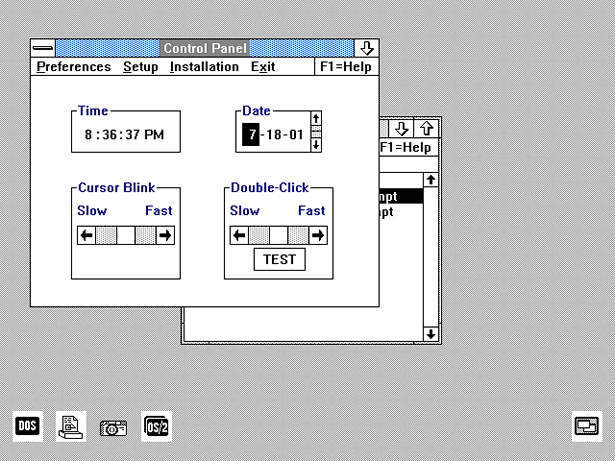
\includegraphics[keepaspectratio]{media/C03_historia/os_2_1.png}
\caption{Panel de control de Microsoft-IBM OS/2 1.1 --- Fuente: Michal
Necasek}\label{fig-os-21}
\end{figure}

En los sistemas con \textbf{operación en modo dual} se distingue entre
dos modos de ejecución, de tal forma que solo en el modo en el que se
ejecuta el código del sistema operativo se pueden realizar operaciones
peligrosas. En el otro modo y con menos privilegios, se ejecutan las
aplicaciones de usuario. Para más información, véase el
\hyperref[_operaciuxf3n_en_modo_dual]{???}

La colaboración entre IBM y Microsoft terminó en 1990, entre el
lanzamiento de Windows 3.0 y la de OS/2 1.3. El aumento de popularidad
de Windows llevó a Microsoft a dejar de centrarse en el desarrollo de
OS/2, lo que hizo que IBM se preocupara por los continuos retrasos en el
desarrollo de OS/2 2.0. Inicialmente ambas compañías acordaron que IBM
tomaría el mantenimiento de OS/2 1.0 y el desarrollo de OS/2 2.0,
mientras Microsoft continuaría desarrollando OS/2 3.0, que entonces era
conocido como «NT OS/2». Sin embargo, Microsoft finalmente decidió
renombrar NT OS/2 como Windows NT, dejando el futuro desarrollo de OS/2
en manos de IBM.

OS/2 Warp 3 fue un sistema completo de 32 bits lanzado en 1994. Le
seguiría OS/2 Warp 4, en 1996. Poco después, IBM anunció que OS/2
desaparecería.

\subsection{Windows 3.x}\label{_windows_3_x}

La familia \href{https://es.wikipedia.org/wiki/Windows_3.1x}{Windows
3.x} de Microsoft Windows fue desarrollada desde 1990 hasta 1994.
Windows 3.0 fue la primera versión de éxito de Windows, permitiendo a
Microsoft competir con el
\href{https://es.wikipedia.org/wiki/Macintosh}{Macintosh} de Apple
Computer y el
\href{https://es.wikipedia.org/wiki/Commodore_Amiga}{Commodore Amiga}.

\begin{figure}
\centering
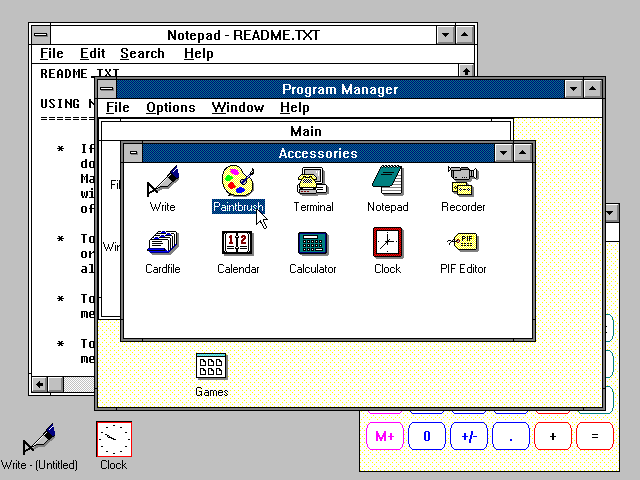
\includegraphics[keepaspectratio]{media/C03_historia/windows_30.png}
\caption{Administrador de programas de Microsoft Windows 3.0 --- Fuente:
\href{https://guidebookgallery.org/screenshots/win30}{Guidebook}}\label{fig-windows-30}
\end{figure}

En 1983, Microsoft anunció el desarrollo de Windows, una interfaz
gráfica de usuario para su sistema MS-DOS, que se usaba en los IBM PC y
compatibles desde 1981. Windows requería una instalación previa de
MS-DOS y era iniciado como un programa más, que podía ser terminado en
cualquier momento, devolviendo al usuario a la línea de comandos de
MS-DOS.

MS-DOS le proporcionaba a Windows controladores de dispositivo para
ciertas tareas, como el acceso al CD-ROM o a la interfaz de red. Sin
embargo Windows ejecutaba aplicaciones específicas de Windows,
almacenadas en un formato ejecutable mucho más complejo que el de los
programas de MS-DOS. Además, debido a que MS-DOS no aislaba a las
aplicaciones del hardware y no se protegía así mismo de los errores en
dichas aplicaciones, Windows disponía de controladores de dispositivo
propios, así como sus propios sistemas de gestión de procesos y de
memoria. En realidad Windows no se ejecutaba sobre MS-DOS, si no que
hacía uso de él. Por ello puede ser considerado como un sistema
operativo.

\subsection{Windows 95, 98, Me}\label{_windows_95_98_me}

La familia Windows 3.x fue sustituida por una serie de sistemas
operativos gráficos híbridos de 16/32 bits.

\begin{figure}
\centering
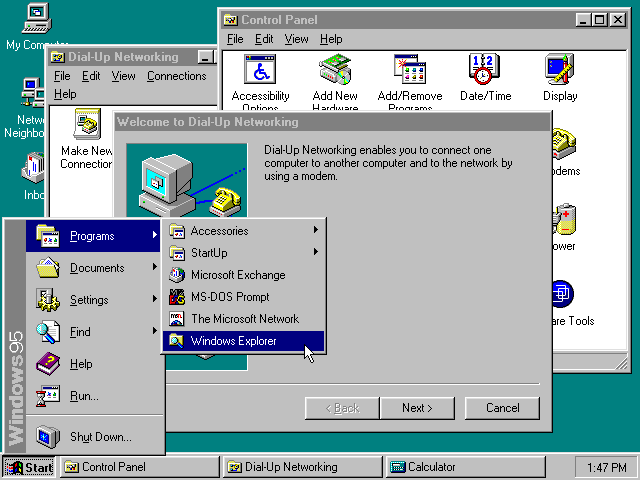
\includegraphics[keepaspectratio]{media/C03_historia/windows_95.png}
\caption{Escritorio de Microsoft Windows 95 --- Fuente:
\href{http://www.guidebookgallery.org/screenshots/win95}{Guidebook}}\label{fig-windows-95}
\end{figure}

Windows 95 fue lanzado en 1995. Fue el primer Windows unido a una
versión de MS-DOS específica, aunque este hecho se intentaba mantener
oculto. Entre las características de Windows 95 destacan: mejoras
significativas en la interfaz de usuario (véase la
\hyperref[fig-windows-95]{Escritorio de Microsoft Windows 95 --- Fuente:
}), nombres de archivo de hasta 256 caracteres con conservación de
mayúsculas y minúsculas ---en MS-DOS el límite era de 8 caracteres para
el nombre más 3 de extensión--- y multitarea expropiativa para las
aplicaciones de 32 bits.

Como veremos en el \hyperref[_planificaciuxf3n_expropiativa]{???}, la
planificación expropiativa es una técnica que permite al sistema
operativo expulsar de la CPU a los procesos en ciertas circunstancias;
como, por ejemplo, que llevan demasiado tiempo utilizando la CPU de
forma ininterrumpida.

En la familia Windows 3.x la planificación era cooperativa, es decir,
los procesos abandonaban la CPU voluntariamente. Esto ocasionaba
problemas con programas que no devolvía la CPU al sistema con la
suficiente frecuencia, ya que así el resto de procesos no tenía ocasión
de ejecutarse para hacer su trabajo o responder al usuario.

Windows 98 fue lanzado el 25 de junio de 1998. Le siguió Windows Me, el
14 de septiembre de 2000. Windows Me fue la última versión de la familia
de sistemas operativos híbridos de 16/32 bits que sucedió a la familia
Windows 3.x.

\subsection{Windows NT, 2000, XP, Vista, 7, 8 y
10}\label{sect-windows-nt}

Windows NT fue un sistema operativo de 32 bits. El primero de la familia
de sistemas operativos Microsoft Windows actuales.

Su desarrollo empezó en 1988 con el nombre de OS/2 3.0. Cuando Windows
3.0 fue lanzado en mayo de 1990, tuvo tanto éxito que Microsoft decidió
cambiar la API del aún en desarrollo NT OS/2 ---que era como Microsoft
lo llamaba entonces--- pasando de ser una versión extendida de la API de
OS/2 a una versión extendida de la API de Windows 3.0. Esta decisión
causó tensión entre Microsoft e IBM y provocó que finalmente terminara
la colaboración.

Una interfaz de programación de aplicaciones o API (del inglés
\emph{Application Programming Interface}) es el conjunto de funciones,
procedimientos o métodos que ofrece el sistema operativo para ser
utilizado por las aplicaciones.

Como hemos comentado anteriormente, Microsoft contrató a un grupo de
desarrolladores de Digital Equipment Corporation para crear Windows NT.
Por lo que muchos de sus elementos reflejan la experiencia anterior de
DEC en VMS.

Windows NT soportaba varias API de distintos sistemas operativos ---por
ejemplo Win32, POSIX y OS/2 2.1--- que eran implementadas como
subsistemas encima de una API nativo no documentado públicamente. Esta
estructura en subsistemas, fue lo que permitió la adopción tardía de la
API de Windows 3.0 como API principal, tal y como hemos comentado.

La primera versión ---Windows NT 3.1--- lanzada el 13 de julio de 1993,
era un sistema operativo \emph{microkernel} (véase el
\hyperref[_mach]{Mach} un poco más adelante) multiplataforma que corría
sobre procesadores \{x86\}, \{decalpha\}, \{mips\} 4000 y
\href{https://es.wikipedia.org/wiki/PowerPC}{PowerPC}.

Windows NT 4.0 ---lanzado en 1996--- fue la última versión en soportar
plataformas distintas a Intel IA-32. Aunque el desarrollo de Windows
2000 para procesador Alpha continuó un poco más, hasta 1999, cuando
Compaq dejó de soportar Windows NT en esa arquitectura. Además Windows
NT 4.0 integró en el núcleo más funciones ---por ejemplo, parte del
subsistema gráfico--- para obtener un rendimiento más próximo al de
Windows 95 en ese apartado.

Windows 2000 ---o Windows NT 5.0--- fue lanzado el 17 de febrero de 2000
y fue el primer sistema operativo de la familia NT al que se le
eliminaron las siglas del nombre. Fue por motivos de marketing, para
favorecer la unificación de las dos familias de sistemas operativos
Microsoft Windows de entonces ---Windows 9x y Windows NT--- alrededor de
la tecnología NT.

Windows XP ---o Windows NT 5.1--- completó en 2001 el proceso de
unificación de las dos familias de sistemas operativos Windows. Con su
aparición forzó la extinción de la familia Windows 9x, al sustituirla
con una versión de Windows XP denominada Windows XP Home Edition,
específica para la informática doméstica.

\subsection{GNU/Linux}\label{_gnulinux}

\{gnulinux\} es un sistema operativo libre y, tal vez, el más famoso
proyecto de \href{https://es.wikipedia.org/wiki/Software_libre}{software
libre}.

El proyecto GNU se inició en 1983, con el fin de desarrollar un sistema
operativo estilo UNIX enteramente libre. El proyecto incluía la creación
de herramientas de desarrollo de software y aplicaciones de usuario.

Mucho tiempo después, el estudiante universitario finés Linus Torvalds
comenzó a desarrollar el núcleo Linux como hobby, mientras estudiaba en
la Universidad de Helsinki. Torvalds originalmente usaba \{minix\}, un
sistema operativo simplificado escrito por Andrew Tanenbaum para enseñar
diseño de sistemas operativos. Sin embargo, el hecho de que Tanenbaum no
diera soporte a las mejoras del sistema operativo que eran propuestas
por otros desarrolladores, llevó a Torvalds a escribir un sustituto de
MINIX.

En 1991, cuando se liberó la primera versión del núcleo Linux, el
proyecto GNU había desarrollado todos los componentes necesarios del
sistema operativo excepto el núcleo. Torvalds y otros desarrolladores
rápidamente adaptaron Linux para que funcionara con los componentes de
GNU, creando un sistema operativo completamente funcional que se
denomina GNU/Linux.

El núcleo Linux fue licenciado bajo la GNU General Public License (GPL),
como el resto del proyecto GNU. Pero Linux no es parte de dicho
proyecto. El proyecto GNU tiene su propio núcleo, denominado
\{gnuhurd\}, que lleva 30 años en desarrollo y parece que aún está muy
lejos de estar listo.

GNU no es el único sistema operativo que utiliza el núcleo Linux.
\{android\}, por ejemplo, es un sistema operativo que usa el núcleo
Linux, pero no es GNU.

\subsection{Mach}\label{_mach}

\{mach\} es un núcleo de sistema operativo desarrollado en la
Universidad Carnegie-Mellon (CMU). El proyecto en la CMU se desarrolló
desde 1985 hasta 1994.

Mach explora el concepto que denominamos \textbf{\emph{microkernel}}. En
los sistemas operativos \textbf{\emph{microkernel}} solo se implementa
en el núcleo del sistema un conjunto mínimo de servicios básicos. El
resto de los servicios proporcionados por el sistema operativo se
implementan como procesos con menos privilegios.

Por sus ventajas en cuanto a seguridad y fiabilidad, en algún momento se
pensó que los \emph{microkernel} dominarían el universo de los sistemas
operativos. Sin embargo, el mayor esfuerzo hasta la fecha para
conseguirlo es \{gnuhurd\}, que lleva varias décadas de retraso. Por
fortuna, otros sistemas operativos \emph{microkernel} han tenido algo
más éxito, como es el caso de \{qnx\} o \{minix3\}. Mientras que Google
parece que lo va a intentar con \{google\_fuchsia\}, el posible
sustituto de Android.

A mediados de los 90, Apple Computers seleccionó
\href{https://es.wikipedia.org/wiki/NEXTSTEP}{OpenStep} como base para
el sucesor de su clásico
\href{https://es.wikipedia.org/wiki/Mac_OS_Classic}{Mac OS}. OpenStep es
realmente una versión actualizada de NeXTSTEP que era un sistema basado
en un núcleo Mach 2.5 con porciones del sistema UNIX BSD de la
Universidad de Berkeley. Por tanto, la mezcla de Mach con UNIX BSD de
OpenStep es la base del sistema operativo \{macos\} actual de Apple.

\begin{figure}
\centering
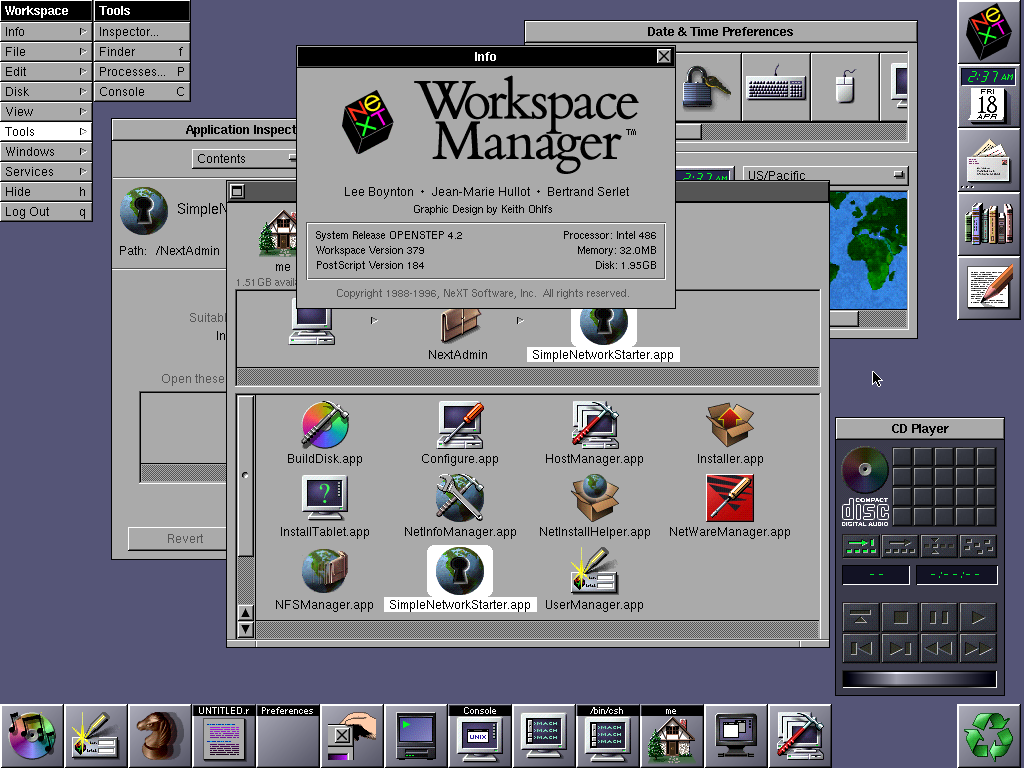
\includegraphics[keepaspectratio]{media/C03_historia/openstep_42.png}
\caption{Entorno gráfico de OpenStep 4.2 --- Fuente:
\href{https://guidebookgallery.org/screenshots/openstep42}{Guidebook}}\label{fig-openstep-42}
\end{figure}

Para ser exactos, la base del sistema operativo macOS es un sistema
operativo libre denominado \{darwin\} y desarrollado por Apple. Se trata
de un sistema \{freebsd\} adaptado para correr sobre el núcleo Mach.

\begin{figure}
\centering
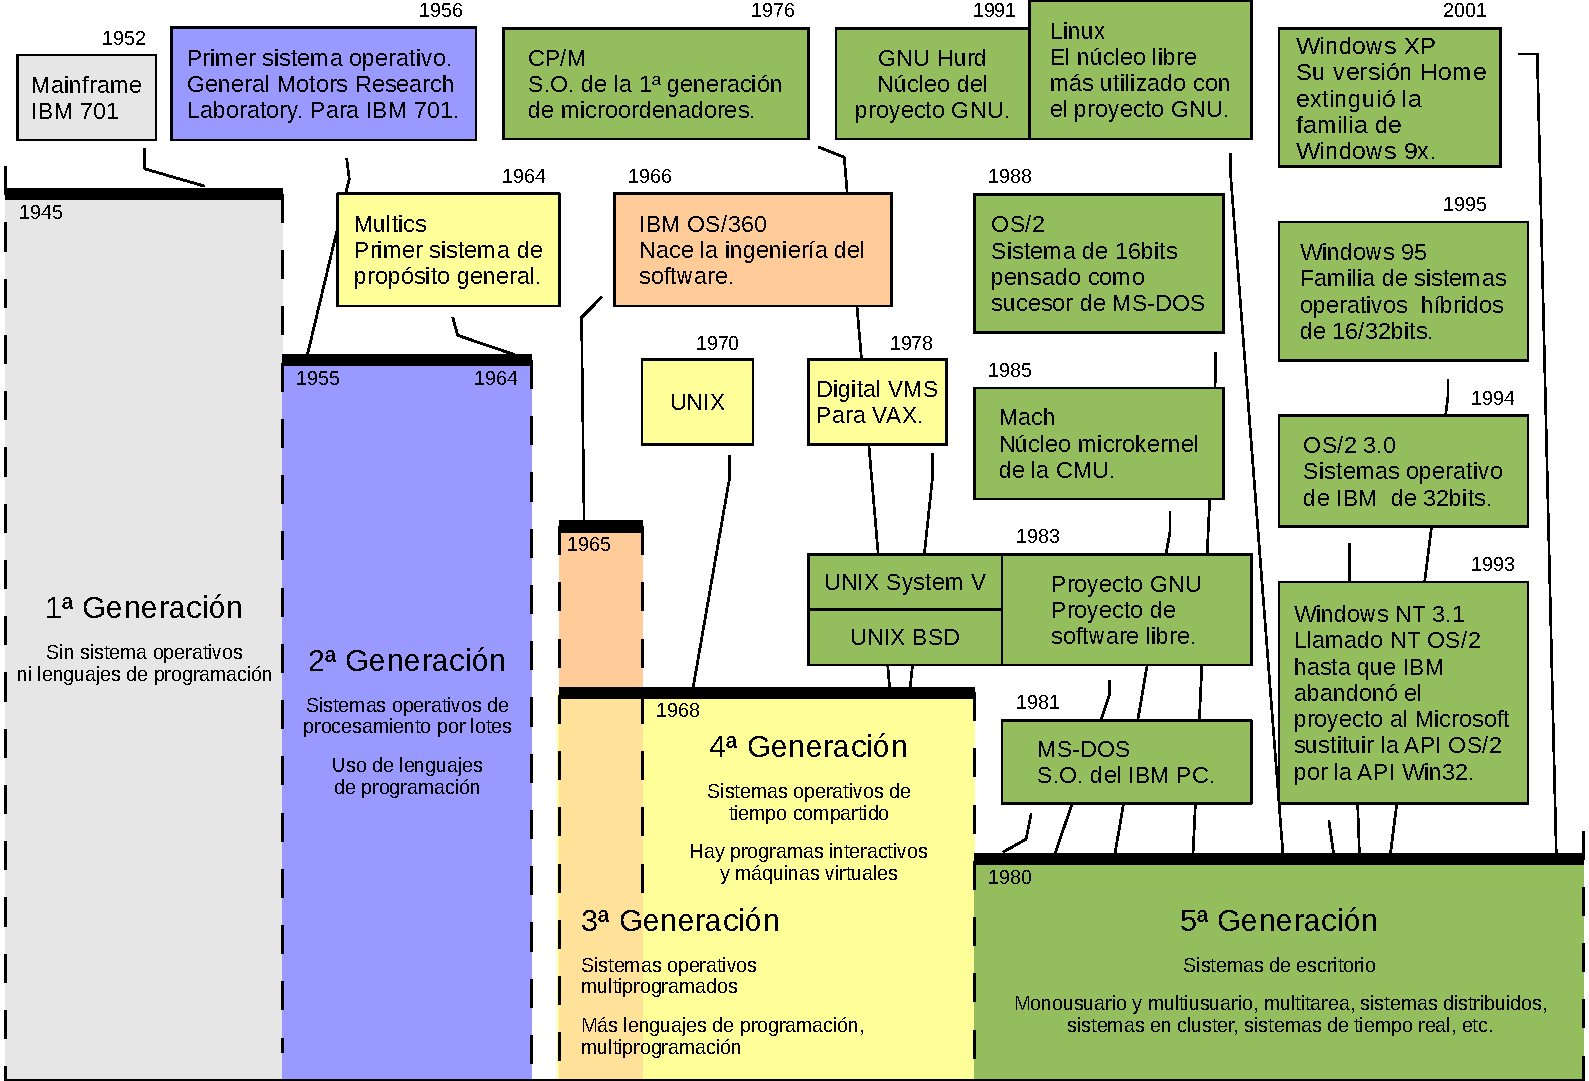
\includegraphics[width=0.8\textwidth]{media/C03_historia/historia_sistemas_operativos.pdf}
\caption{Línea de tiempo de la historia de los sistemas operativos.}
\end{figure}
